\documentclass[twocolumn]{report}
\usepackage[margin=1in]{geometry}
\usepackage{amsmath}
\usepackage{amssymb}
\usepackage{subfiles}

\title{ENGT 3652 Project 3:\\*Threaded Bolt Circles}
\author{Leomar Dur\'an}
\date{${27}^{\text{th}}$ April 2023}

\usepackage{pdflscape}
\usepackage{graphicx}
\usepackage{minted}
\newcommand*\gcode{lib/pygments/gcodelexer.py:GcodeLexer -x}

%\usepackage[final]{pdfpages}
%\write18{
%    % the manual gcode for CNC Simulator in two columns
%    pdflatex gcode-cam
%}
% usage: \includepdf[pages=2-,pagecommand={}]{gcode-cam.pdf}

\begin{document}

\maketitle

\chapter{Verification of operations in MasterCAM}
\onecolumn
    \begin{landscape}
        \null\vfill
        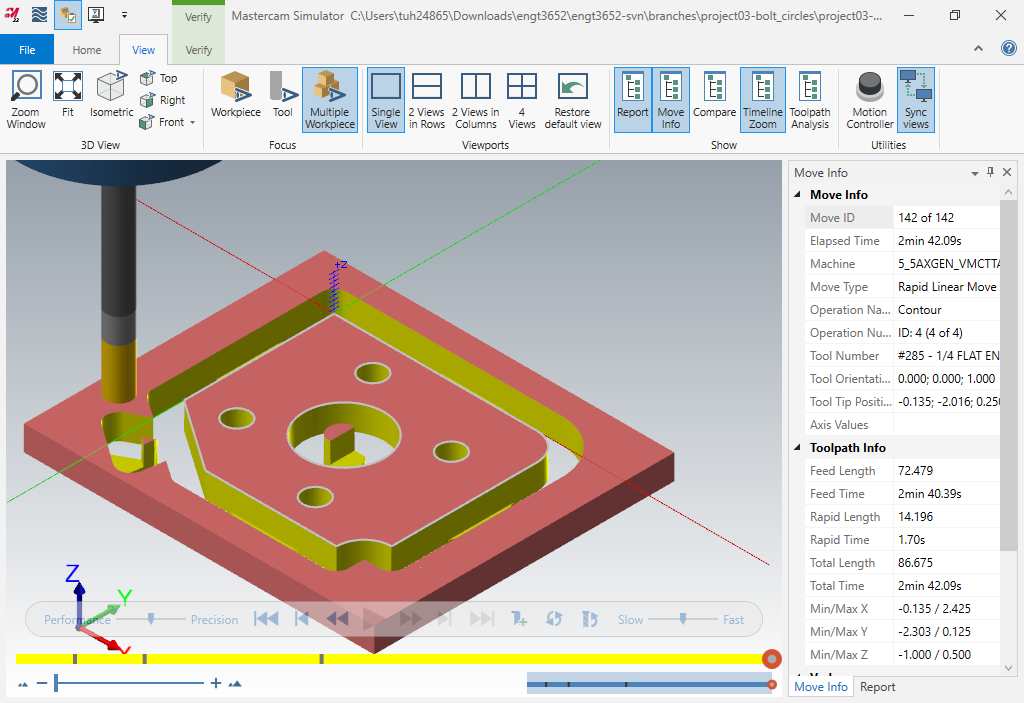
\includegraphics[width=\linewidth]{img/prj03-mastercam_simulator-verification.png}
        \vfill
    \end{landscape}
\twocolumn

\chapter{The MasterCAM-generated Gcode}
\inputminted[breaklines]\gcode{src/boltCircles.NC}

\chapter{Plot of MasterCAM-generated Gcode in NCViewer}
\onecolumn
    \begin{landscape}
        % this image has a lower portrait aspect ratio than a page, so use height for reference
        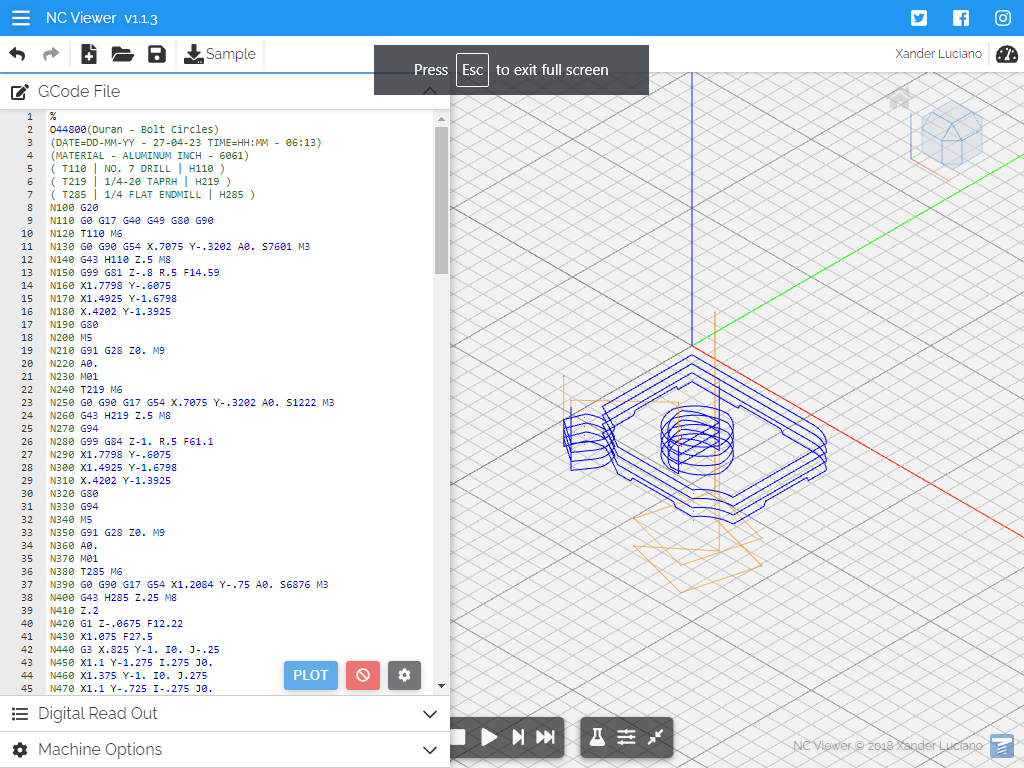
\includegraphics[height=\textheight]{img/prj03-cam-gcode-ncviewer-plot.png}
    \end{landscape}
\twocolumn

\onecolumn
    \chapter{The machined part}
    \null\vfill
    \centering\includegraphics[width=\linewidth]{img/machined-03-bolt_circles.png}
    \vfill
\twocolumn

\end{document}
